%%%%%%%%%%%%%%%%%%%%%%%%%%%%%%%%%%%%%%%%%%%%%%%%%%%%%%%%%%%%%%%%%%%%%%%%%%%%%%%
%                       CARREGA DE LA CLASSE DE DOCUMENT                      %
%                                                                             %
% Les opcions admissibles son:                                                %
%      12pt / 11pt            (cos dels tipus de lletra; no feu servir 10pt)  %
%                                                                             %
% catalan/spanish/english     (llengua principal del treball)                 %
%                                                                             % 
% french/italian/german...    (si necessiteu fer servir alguna altra llengua) %
%                                                                             %
% listoffigures               (El document inclou un Index de figures)        %
% listoftables                (El document inclou un Index de taules)         %
% listofquadres               (El document inclou un Index de quadres)        %
% listofalgorithms            (El document inclou un Index d'algorismes)      %
%                                                                             %
%%%%%%%%%%%%%%%%%%%%%%%%%%%%%%%%%%%%%%%%%%%%%%%%%%%%%%%%%%%%%%%%%%%%%%%%%%%%%%%

\documentclass[11pt,spanish,listoffigures,listoftables]{tfgetsinf}

%%%%%%%%%%%%%%%%%%%%%%%%%%%%%%%%%%%%%%%%%%%%%%%%%%%%%%%%%%%%%%%%%%%%%%%%%%%%%%%
%                     CODIFICACIO DEL FITXER FONT                             %
%                                                                             %
%    windows fa servir normalment 'ansinew'                                   %
%    amb linux es possible que siga 'latin1' o 'latin9'                       %
%    Pero el mes recomanable es fer servir utf8 (unicode 8)                   %
%                                          (si el vostre editor ho permet)    % 
%%%%%%%%%%%%%%%%%%%%%%%%%%%%%%%%%%%%%%%%%%%%%%%%%%%%%%%%%%%%%%%%%%%%%%%%%%%%%%%

\usepackage[utf8]{inputenc} 

%%%%%%%%%%%%%%%%%%%%%%%%%%%%%%%%%%%%%%%%%%%%%%%%%%%%%%%%%%%%%%%%%%%%%%%%%%%%%%%
%                        ALTRES PAQUETS I DEFINICIONS                         %
%                                                                             %
% Carregueu aci els paquets que necessiteu i declareu les comandes i entorns  %
%                                          (aquesta seccio pot ser buida)     %
%%%%%%%%%%%%%%%%%%%%%%%%%%%%%%%%%%%%%%%%%%%%%%%%%%%%%%%%%%%%%%%%%%%%%%%%%%%%%%%
\usepackage{amsmath}
\usepackage{tikz}
\usetikzlibrary{positioning}
\usetikzlibrary{babel}
\usepackage{hyperref}
\usepackage{csquotes}

%%%%%%%%%%%%%%%%%%%%%%%%%%%%%%%%%%%%%%%%%%%%%%%%%%%%%%%%%%%%%%%%%%%%%%%%%%%%%%%
%                        DADES DEL TREBALL                                    %
%                                                                             %
% titol, alumne, tutor i curs academic                                        %
%%%%%%%%%%%%%%%%%%%%%%%%%%%%%%%%%%%%%%%%%%%%%%%%%%%%%%%%%%%%%%%%%%%%%%%%%%%%%%%

\title{Adaptación de modelos de lenguaje grandes para la generación
de lenguaje natural a partir de palabras clave en sistemas
aumentativos y alternativos de comunicación}
\author{Silvia Alegre Villa}
\tutor{Jorge Civera Saiz}
\curs{2023-2024}

%%%%%%%%%%%%%%%%%%%%%%%%%%%%%%%%%%%%%%%%%%%%%%%%%%%%%%%%%%%%%%%%%%%%%%%%%%%%%%%
%                     PARAULES CLAU/PALABRAS CLAVE/KEY WORDS                  %
%                                                                             %
% Independentment de la llengua del treball, s'hi han d'incloure              %
% les paraules clau i el resum en els tres idiomes                            %
%%%%%%%%%%%%%%%%%%%%%%%%%%%%%%%%%%%%%%%%%%%%%%%%%%%%%%%%%%%%%%%%%%%%%%%%%%%%%%%

\keywords{????, ?????????, ????, ?????????????????} % Paraules clau 
         {?????, ???, ???????????????}              % Palabras clave
         {?????, ????? ?????, ?????????????}        % Key words

%%%%%%%%%%%%%%%%%%%%%%%%%%%%%%%%%%%%%%%%%%%%%%%%%%%%%%%%%%%%%%%%%%%%%%%%%%%%%%%
%                              INICI DEL DOCUMENT                             %
%%%%%%%%%%%%%%%%%%%%%%%%%%%%%%%%%%%%%%%%%%%%%%%%%%%%%%%%%%%%%%%%%%%%%%%%%%%%%%%

\begin{document}

%%%%%%%%%%%%%%%%%%%%%%%%%%%%%%%%%%%%%%%%%%%%%%%%%%%%%%%%%%%%%%%%%%%%%%%%%%%%%%%
%              RESUMS DEL TFG EN VALENCIA, CASTELLA I ANGLES                  %
%%%%%%%%%%%%%%%%%%%%%%%%%%%%%%%%%%%%%%%%%%%%%%%%%%%%%%%%%%%%%%%%%%%%%%%%%%%%%%%

\begin{abstract}
Els Sistemes Augmentatius i Alternatius de Comunicació (SAAC) son eines essencials per a facilitar la comunicació de les persones amb dificultats en la utilització del llenguatge. Aquest sistemes permeten a l'usuari la selecció de pictogrames associats a paraules claus que conformaran l'oració que es desitja comunicar. Posteriorment, aquesta oració pot ser sintetitzada amb veu humana. Els recents avanços en l'àrea del processament del llenguatge natural i, en concret, la proliferació de models de llenguatge grans ofereixen noves perspectives per a millorar els SAAC. En particular, aquest treball explorarà com aquests models de llenguatge poden millorar l'expressivitat de la comunicació dels SAAC quan s'utilitzen per a la generació de llenguatge natural a partir de les paraules clau (pictogrames) seleccionades per l'usuari. D'aquesta manera, aquest treball evaluar'a el rendiment d'aquests models quan són adaptats per a la seua integració en els SAAC. Awuesta evaluació es durà a terme utilitzant conjunts de test reals en espanyol i anglés extrets del portal del Centre Aragonés per a la Comunicació Augmentativa i Alternativa.
\end{abstract}
\begin{abstract}[spanish]
 Los Sistemas Aumentativos y Alternativos de Comunicación (SAAC) son herramientas vitales para facilitar la comunicación de las personas con dificultades en la utilización del lenguaje. Estos sistemas permiten al usuario la selección de pictogramas asociados a palabras clave que conformarán la oración que se desea comunicar. Posteriormente, esta oración puede ser sintetizada con voz humana. Los recientes avances en el área del procesamiento de lenguaje natural y, en concreto, la proliferación de modelos de lenguaje grandes ofrece nuevas perspectivas para mejorar los SAAC. En particular, este trabajo explorará cómo estos modelos de lenguaje pueden mejorar la expresividad de la comunicación de los SAAC cuando se utilizan para la generación de lenguaje natural a partir de las palabras clave (pictogramas) seleccionadas por el usuario. De esta forma, este trabajo evaluará el rendimiento de estos modelos cuando son adaptados para su integración en los SAAC. Esta evaluación se llevará a cabo utilizando conjuntos de test reales en español e inglés extraídos del portal del Centro Aragonés para la Comunicación Aumentativa y Alternativa.
\end{abstract}
\begin{abstract}[english]
Augmentative and Alternative Communication (AAC) systems are vital tools for facilitating communication for individuals with difficulties using language. These systems allow users to select pictograms associated with key words that will form the sentence that is wished to communicate. Then, the sentence can be synthesized with a human voice. Recent advances in the field of natural language processing, and specifically the proliferation of large language models, offer new perspectives for improving AAC systems. In particular, this work will explore how these language models can enhance the expressiveness of AAC communication when used to generate natural language from the key words (pictograms) selected by the user. In this way, this work will evaluate the performance of these models when adapted for integration into AAC systems. This evaluation will be carried out using real test sets in spanish and english extracted from the portal of the Aragonese Center for Augmentative and Alternative Communication.
\end{abstract}

%%%%%%%%%%%%%%%%%%%%%%%%%%%%%%%%%%%%%%%%%%%%%%%%%%%%%%%%%%%%%%%%%%%%%%%%%%%%%%%
%                              CONTINGUT DEL TREBALL                          %
%%%%%%%%%%%%%%%%%%%%%%%%%%%%%%%%%%%%%%%%%%%%%%%%%%%%%%%%%%%%%%%%%%%%%%%%%%%%%%%

\mainmatter

%%%%%%%%%%%%%%%%%%%%%%%%%%%%%%%%%%%%%%%%%%%%%%%%%%%%%%%%%%%%%%%%%%%%%%%%%%%%%%%
%                                  INTRODUCCIO                                %
%%%%%%%%%%%%%%%%%%%%%%%%%%%%%%%%%%%%%%%%%%%%%%%%%%%%%%%%%%%%%%%%%%%%%%%%%%%%%%%

\chapter{Introducción}
ESCRIBIR BIEN !!!
En este primer capítulo introductorio presentamos la motivación y objetivos del trabajo. También explicaremos cómo será la estructura del contenido de este.

\section{Motivación}

La comunicación y el lenguaje son dos pilares fundamentales de la sociedad actual, pues constituyen la base de las relaciones interpersonales, permitiendo el intercambio de ideas e información. Gracias a ello podemos transmitir a los demás nuestros pensamientos, emociones y necesidades, permitiéndonos participar en la vida en sociedad. Sin embargo, para algunas personas, el hecho de comunicarse de manera satisfactoria puede resultar realmente complicado debido a distintas causas. Es aquí donde entran en juego los Sistemas Aumentativos y Alternativos de Comunicación (SAAC).

Tal y como explica el Centro Aragonés para la Comunicación Aumentativa y Alternativa (ARASAAC), “los Sistemas Aumentativos y Alternativos de Comunicación son formas de expresión distintas al lenguaje hablado que tienen como objetivo aumentar el nivel de expresión y/o compensar las dificultades de comunicación y lenguaje de las personas que tienen dificultades en este ámbito”. Hay distintas razones por las cuales una persona podría necesitar utilizar un SAAC. Entre ellas encontramos la parálisis cerebral, la discapacidad intelectual, los trastornos del espectro autista, algunas enfermedades neurológicas, las distrofias musculares o las afasias, entre otras.

Aunque hay muchos tipos de SAAC, todos se caracterizan por estar basados en sistemas de símbolos, ya sean gráficos (fotografías, dibujos, pictogramas, palabras o letras) o gestuales (mímica o símbolos manuales). En este trabajo nos centraremos en los comunicadores electrónicos. Los comunicadores electrónicos son herramientas tecnológicas que pueden ser utilizados en cualquier tipo de dispositivo electrónico. Por lo general, consisten en un tablero donde aparecen distintos símbolos gráficos (pictogramas) que representan palabras.

\begin{figure}[h]
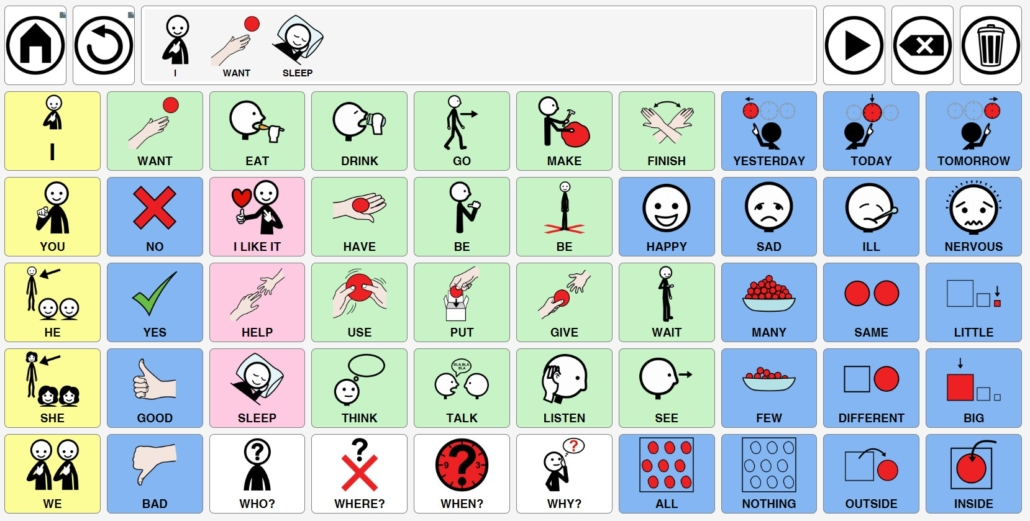
\includegraphics[scale = 0.5]{images/asteriscsGrid.jpg}
\centering
\caption{Comunicador AsTeRISCS Grid desarrollado por ARASAAC}
\end{figure}

Estos pictogramas pueden ser organizados y adaptados dependiendo de las necesidades de cada persona, permitiendo que cada usuario añada aquellos que necesite. El funcionamiento es simple: el usuario clica sobre los pictogramas y el programa se encarga de dar la salida del mensaje, generalmente en forma de habla digitalizada o en formato escrito.

Así, estas herramientas resultan verdaderamente útiles para solventar los problemas de comunicación de las personas. Sin embargo, presentan una limitación que puede afectar a la fluidez y al nivel de expresividad con que se realiza la comunicación: la dificultad para conjugar las frases de manera adecuada, pues para facilitar y simplificar el uso de la herramienta, en este tipo de tableros se suelen incluir solamente palabras clave en su forma simple, sin distinción de número, género o tiempo verbal.

Algunos de los comunicadores que existen actualmente en el mercado ya emplean diferentes métodos para abordar este problema, pero existe todavía un amplio margen de mejora. Los modelos de lenguaje grandes prometen ofrecer buenos resultados en este área.


\section{Objetivos}

Los objetivos de este proyecto son los siguientes:
\begin{enumerate}
\item Investigar sobre los enfoques actuales para la generación de frases en el sector de los SAAC.
\item Implementar y evaluar modelos de lenguaje grandes para este tipo de herramientas.
\item Comparar los resultados que se obtienen con los modelos de lenguaje grandes respecto a otros comunicadores que permiten la generación de frases que se encuentran en el mercado, utilizando para ello las métricas de BLEU y COMET.
\end{enumerate}

\section{Estructura de la memoria}

????? ????????????? ????????????? ????????????? ????????????? ????????????? 

%\section{Notes bibliografiques} %%%%% Opcional

%????? ????????????? ????????????? ????????????? ????????????? ?????????????

%%%%%%%%%%%%%%%%%%%%%%%%%%%%%%%%%%%%%%%%%%%%%%%%%%%%%%%%%%%%%%%%%%%%%%%%%%%%%%%
%                         CAPITOLS (tants com calga)                          %
%%%%%%%%%%%%%%%%%%%%%%%%%%%%%%%%%%%%%%%%%%%%%%%%%%%%%%%%%%%%%%%%%%%%%%%%%%%%%%%

\chapter{Fundamentos}\label{capitulo:fundamentos}

REESCRIBIR: Los modelos de lenguaje se encuadran dentro de las técnicas de procesamiento de lenguaje natural, las cuales forman parte del ámbito del aprendizaje automático. Antes de profundizar en las tareas específicas que realizan los modelos de lenguaje grandes, debemos introducir los conceptos básicos del aprendizaje automático, del aprendizaje profunod y del procesamiento de lenguaje natural. Así, en este capítulo abordaremos las distintas tareas y enfoques del aprendizaje automático, proporcionando el contexto necesario para comprender el funcionamiento y las aplicaciones de los modelos de lenguaje.

\section{Aprendizaje automático}

El aprendizaje automático (en inglés, \textit{machine learning}) es una disciplina dentro de la inteligencia artificial que se centra en el desarrollo y estudio de algoritmos y modelos que permiten que los sistemas puedan relizar tareas específicas sin haber sido explícitamente programados para ello. Este término fue acuñado por Arthur Samuel en el año 1959, quien creo uno de los primeros programas exitosos de esta disciplina, conocido como \textit{the Samuel Ckeckers-playing Program} \cite{samuelCheckers} (el programa de juego de damas de Samuel).

Tom Mitchell \cite{mitchell1997mcgraw} define el proceso de aprendizaje de los programas en el campo del \textit{machine learning} de la siguiente manera:

\begin{displayquote}
\textit{"Se dice que un programa aprende de la experiencia $E$ con respecto a alguna clase de tarea $T$, y medida de rendimiento $P$, si su rendimiento en tareas en $T$, medido por $P$, mejora con la experiencia $E$."}
\end{displayquote}

Aunque la idea principal del aprendizaje automático es esta, econtramos diferentes tipos de aprendizaje automático, dependiendo del tipo de tarea que se quiera llevar a cabo, de la naturaleza de la medida del rendimiento que se utiliza para evaluar el sistema y de el tipo de entrenamiento o experiencia que le proporcionamos a este.

Generalmente, los enfoques para el entrenamiento de algoritmos se agrupan en:

\begin{itemize}
	\item \textbf{Aprendizaje supervisado}, cuyo objetivo es, a partir de unos datos de entrenamiento, encontrar la función $f$ que realice el mejor mapeo posible entre un conjunto de entradas $X$ y sus salidas correspondientes $Y$, de manera que $(X, Y) = (X, f(Y))$
	\item \textbf{Aprendizaje no supervisado}, que trata de modelar la estructura subyacente de un conjunto de datos para identificar relaciones y patrones, permitiendo así un entendimiento más profundo de los mismos
	\item \textbf{Aprendizaje semi-supervisado}, que cae entre el supervisado y el no supervisado y utiliza una porción de datos etiquetados y no etiquetados
	\item \textbf{Aprendizaje por refuerzo}, donde el algoritmo aprende a través de retroalimentaciones que va recibiendo, ajustando sus acciones con el objetivo de maximizar una recompensa acumulada a lo largo del tiempo. \cite{mirtaheri2022machine}

\end{itemize}

La tarea principal de este trabajo se llevará a cabo utilizando técnicas de aprendizaje supervisado.

Otro concepto importante dentro del aprendizaje automático es el aprendizaje profundo (\textit{deep learning}). El aprendizaje profundo es subconjunto dentro del aprendizaje automático que emplea algoritmos basados en redes neuronales. Dentro de este encontramos métodos como las redes neuronales profundas, las redes neuronales recurrentes, las redes neuronales convulacionales y los transformers, entre otros. Estos métodos tienen aplicaciones significativas en una gran variedad de ámbitos, entre los que se encuentra el procesamiento de lenguaje natural, disciplina en la que se enmarca este trabajo. En las siguientes secciones explicaremos con detalle los conceptos de redes neuronales y transformers.

\section{Redes neuronales}
%https://web.stanford.edu/~jurafsky/slp3/ed3book_jan72023.pdf

El primer modelo de red neuronal artificial fue creado en 1943 por Warren McCulloch y Walter Pitts, y se conoce como \textit{McCulloch-Pitts neuron} \cite{mcculloch1943logical}. Este era un modelo simplificado que imitaba el comportamiento del cerebro humano. A partir de este dio inicio a un proceso de investigación de las redes neuronales desde dos enfoques distintos: uno centrado en los procesos biológicos del cerebro y otro en la aplicación de las redes neuronales para la inteligencia artificial. Las redes neuronales modernas, aunque inspiradas en estas primeras ideas, han evolucionado significatvamente y ya no se basan directamente en las inspiraciones biológicas iniciales.

Las redes neuronales modernas están compuestas por pequeñas unidades de cómputo conocidas como neuronas o nodos, conectadas entre si a través de enlaces para permitir la transmisión de señales entre estas. Los nodos están organizados en capas, de manera que un nodo en una capa está conectado a todos los nodos de la capa siguiente. Existen tres tipos de capa: capa de entrada (\textit{input layer}), capas ocultas (\textit{hidden layers}) y capa de salida (\textit{output layer}). 

La arquitectura más simple de red neuronal es la de perceptrón. Este tipo de modelo se utiliza para tareas de clasificación binaria, en las que se debe decidir si un determinado \textit{input} pertenece o no a una clase. Es un tipo de clasificador lineal, por lo que hace sus predicciones basandose en una función de predicción lineal que combina un conjunto de pesos con el vector de entrada. Este tipo de arquitectura sirve como base para arquitecturas de redes neuronales mucho más complejas.

\begin{figure}[h]
	\centering
	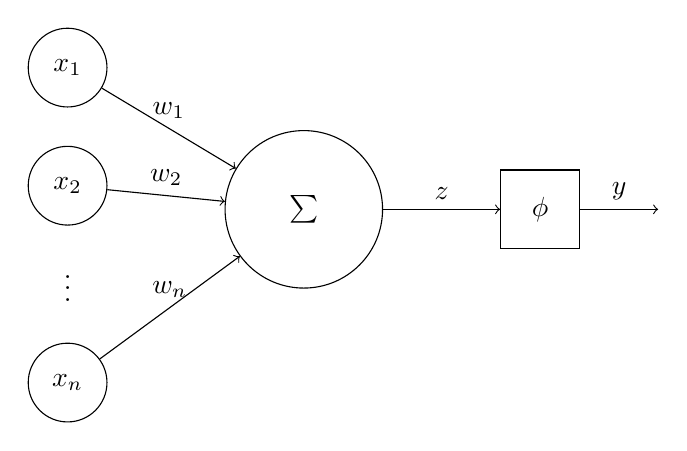
\begin{tikzpicture}
		\tikzstyle{roundnode} = [draw, shape = circle, minimum size = 1cm]
		\tikzstyle{activation} = [draw, shape = rectangle, minimum size = 1cm]
	% Nodos
		\node[roundnode](circle1) at (0, 3.5) {$x_1$};
		\node[roundnode](circle2) at (0, 2) {$x_2$};
		\node (dots) at (0, 0.8) {$\vdots$};
		\node[roundnode](circle3) at (0, -0.5) {$x_n$};

		\node[roundnode, minimum size = 2cm](sum) at (3, 1.7) {$\sum$};
		\node[activation] (act) at (6, 1.7) {$\phi$};

	% Enlaces
		\draw[->]  (circle1) -- (sum) node[midway, above] {$w_1$};
		\draw[->] (circle2) -- (sum) node[midway, above] {$w_2$};
		\draw[->] (circle3) -- (sum) node[midway, above] {$w_n$};
		\draw[->] (sum) -- (act) node[midway, above] {$z$};
		\draw[->] (act) -- (7.5, 1.7) node[midway, above] {$y$};


	\end{tikzpicture}
	\caption{Esquema de perceptrón simple}
\end{figure}


Tal y como vemos en la figura, en la arquitectura de perceptrón encontramos solamente una neurona, que toma un vector $X$ como entrada. La neurona calcula la combinación lineal de los elementos del vector $x_1, x_2, ..., x_n$ con los pesos correspondientes $w_1, w_2, ..., w_n$, añadiendo al resultado un valor conocido como umbral o \textit{bias term}:

 \begin{equation}
\label{form:calcularZ}
z = b + \sum_{i = 1}^n w_i x_i
\end{equation}

 A este resultado se le aplica una función $\phi$ conocida como función de activación, y finalmente se devuelve un solo valor $y$ como salida:

\begin{equation}
y = \phi(z) = 
\begin{cases}
	1 & \text{si } z \ge 0 \\
	0 & \text{si } z < 0
\end{cases}
\end{equation}

El entrenamiento de las redes neuronales consiste en ajustar los distintos pesos de la red de manera que produzca las salidas más acertadas posibles. En el caso de las redes de perceptrón, al contar con solamente una neurona, este proceso resulta relativamente sencillo. El primer paso es inicializar el vector de pesos con valores aleatorios y calcular la salida de cada vector de entrada del conjunto de entrenamiento. A continuación, se comprueba si la predicción ha sido correcta. Si no lo ha sido, el vector de pesos se modifica utilizando la siguiente fórmula:

\begin{equation}
w_i = w_i - \lambda(\hat{Y}^t-Y^t)X^t
\end{equation}

Donde $\lambda$ es la tasa de aprendizaje, $\hat{Y}$ es el \textit{output} predicho por el modelo y $Y$ es la clasificación real.

Estos pasos se repiten durante un número determinado de iteraciones o hasta que el modelo converge.

Este modelo de perceptrón tiene una limitación principal: el modelo solo converge si las dos clases en las cuales debe clasificar las muestras son linealmente separables. En caso de que no lo sean, los pesos oscilarán indefinidamente, hasta que el número máximo de iteraciones se alcance. Para solventar esta limitación existen modelos de redes neuronales mucho más complejos, con más neuronas y que utilizan funciones de activación no lineales. El modelo más conocido de este tipo es el de perceptrón multicapa (MLP, por su nombre en inglés: \textit{Multi-Layer Perceptron}).

\subsection{Perceptrón multicapa} \label{perceptronmulticapa}
El modelo de perceptrón multicapa es una evolución del modelo de perceptrón simple que aparece con intención de poder resolver problemas no lineales. La idea principal detrás de este es la combinación de varios perceptrones simples en un único modelo. En esta arquitectura podemos encontrar un número elevado de neuronas, conectadas entre si y divididas en capas. Encontramos tres tipos de capas: una capa de entrada (\textit{input layer}), una o más capas ocultas (\textit{hidden layers}) y una capa de salida (\textit{output layer}) (ver figura \ref{fig:perceptronMulticapa}).

%\begin{figure}[h]
%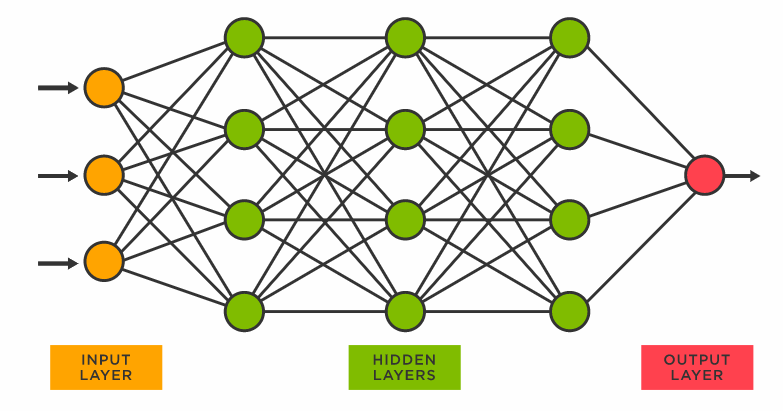
\includegraphics[scale = 0.5]{images/neural_network.png}
%\centering
%\caption{Perceptrón multicapa}
%\end{figure}

\begin{figure}[h]
    \centering
    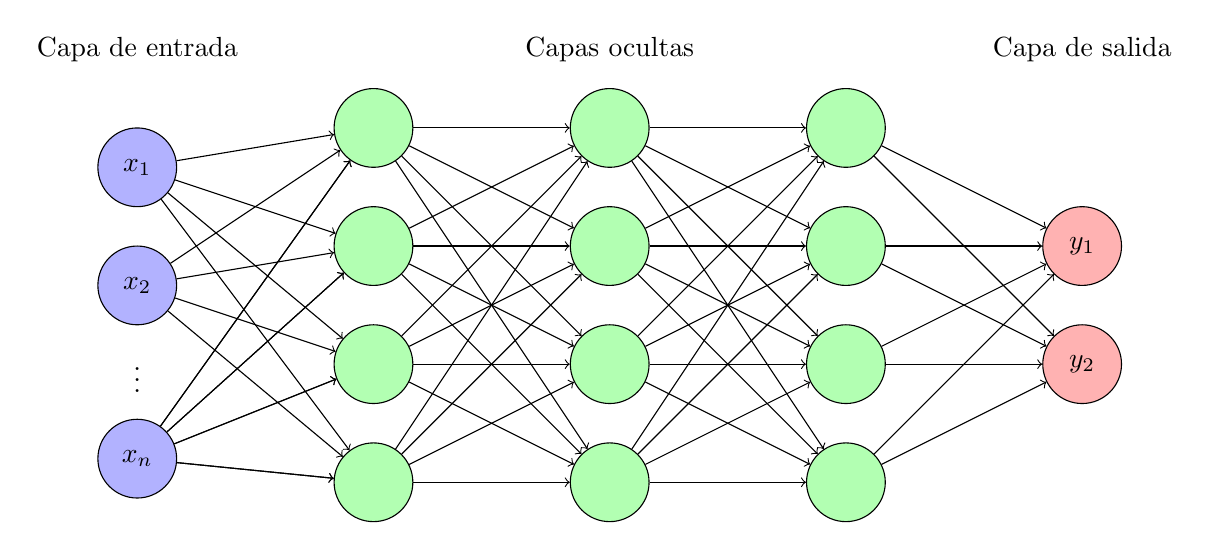
\begin{tikzpicture}
        \tikzstyle{input} = [draw, circle, fill=blue!30, minimum size=1cm]
        \tikzstyle{hidden} = [draw, circle, fill=green!30, minimum size=1cm]
        \tikzstyle{output} = [draw, circle, fill=red!30, minimum size=1cm]
        
        % Nodos de entrada
        \node[input](input1) at (0, 3.5) {$x_1$};
        \node[input](input2) at (0, 2) {$x_2$};
        \node (dots) at (0, 0.9) {$\vdots$};
        \node[input](input3) at (0, -0.2) {$x_n$};

        % Nodos ocultos 1
        \node[hidden](hidden1) at (3, 4) {};
        \node[hidden](hidden2) at (3, 2.5) {};
        \node[hidden](hidden3) at (3, 1) {};
        \node[hidden](hidden4) at (3, -0.5) {};

        % Nodos ocultos 2
        \node[hidden](hidden5) at (6, 4) {};
        \node[hidden](hidden6) at (6, 2.5) {};
        \node[hidden](hidden7) at (6, 1) {};
        \node[hidden](hidden8) at (6, -0.5) {};

        % Nodos ocultos 3
        \node[hidden](hidden9) at (9, 4) {};
        \node[hidden](hidden10) at (9, 2.5) {};
        \node[hidden](hidden11) at (9, 1) {};
        \node[hidden](hidden12) at (9, -0.5) {};

        % Nodos de salida
        \node[output](output1) at (12, 2.5) {$y_1$};
        \node[output](output2) at (12, 1) {$y_2$};

        % Enlaces desde la capa de entrada a la primera capa oculta
        \foreach \i in {1,2,3}
            \foreach \j in {1,2,3,4}
                \draw[->] (input\i) -- (hidden\j);

        \draw[->] (input3) -- (hidden1);
        \draw[->] (input3) -- (hidden2);
        \draw[->] (input3) -- (hidden3);
        \draw[->] (input3) -- (hidden4);
        
        % Enlaces desde la primera capa oculta a la segunda capa oculta
        \foreach \i in {1,2,3,4}
            \foreach \j in {5,6,7,8}
                \draw[->] (hidden\i) -- (hidden\j);

        % Enlaces desde la segunda capa oculta a la tercera capa oculta
        \foreach \i in {5,6,7,8}
            \foreach \j in {9,10,11,12}
                \draw[->] (hidden\i) -- (hidden\j);

        % Enlaces desde la tercera capa oculta a la capa de salida
        \foreach \i in {9,10,11,12}
            \foreach \j in {1,2}
               \draw[->] (hidden\i) -- (output\j);

        % Textos de las capas
        \node at (0, 5) {Capa de entrada};
        \node at (6, 5) {Capas ocultas};
        \node at (12, 5) {Capa de salida};
    \end{tikzpicture}
    \caption{Esquema de perceptrón multicapa}
    \label{fig:perceptronMulticapa}	
\end{figure}

Cada una de las neuronas que se encuentra en una capa está conectada a todas las neuronas de la capa siguiente, y cada uno de los enlaces tiene asociado un peso $w$. De manera similar al modelo de perceptrón simple, los datos entran al modelo en forma de vector a través de la capa de entrada, y se calcula el valor $z_i$ de cada entrada utilizando la fórmula \ref{form:calcularZ}. A continuación se aplica la función de activación $\phi$. Así, el resultado que pasa a la neurona siguiente es $\phi(t)$. En este tipo de modelos se utilizan funciones no lineales como función de activación, para poder aplicarse a problemas no lineales. Entre las funciones de activación más comunes se encuentran la función sigmoide, la tangente hiperbólica (\textit{tanh}) y la rectificada lineal (\textit{ReLU}).

Este proceso se repite en todas las capas, hasta llegar a la capa de salida y producir el \textit{output} final.

\subsection{Redes neuronales para secuencias de texto}

% Probabilistic neural networks (book1)

%En esta sección presentaremos dos tipos de redes neuronales que se utilizan para tareas con secuencias de texto.

El procesamiento de secuencias de texto utilizando redes neuronales es una técnica fundamental en el campo del procesamiento de lenguaje natural. Dado que las redes neuronales operan utilizando vectores numéricos, es necesario transformar las secuencias de texto en vectores antes de poder procesarlas. Este proceso se realiza en varias etapas, que se detallan a continuación:

\begin{enumerate}
	\item \textbf{Tokenización y conversión a índices}: el primer paso consiste en convertir la frase en una secuencia de palabras o tokens. Una vez obtenida la lista de tokens, se asigna a cada uno un número que servirá como índice.
	\item \textbf{Transformación de palabras en vectores}: los índices numéricos se transforman en vectores utilizando \textit{embeddings}. Los \textit{embeddings} son representaciones vectoriales densas y de baja dimensión que capturan las características semánticas de las palabras.
	\item \textbf{Creación de la matriz de \textit{embeddings}}: una vez que se han obtenido los vectores asociados a cada una de las palabras, se puede construir una matriz de \textit{embeddings} que representa la frase completa. Esta matriz facilita la entrada secuencial de los vectores en la red neuronal.
\end{enumerate}

Cada palabra en la secuencia de texto es procesada por la red neuronal de manera secuencial. A continuación, se presentan dos tipos de red neuronal que son utilizadas para el procesamiento de este tipo de datos.

\subsubsection{Redes neuronales recurrentes (RNN)} \label{rnn}
Las redes neuronales recurrentes (en inglés, \textit{recurrent neural networks} (RNN)) son un tipo de red neuronal que mapean desde un conjunto de entrada a otro de salida de manera que la predicción $y_t$ depende no solo de la de entrada $x_t$ sino también del estado oculto del sistema, $h_t$ \cite{murphy2022probabilistic}. El estado oculto $h_t$ es una representación interna de la red en el momento de tiempo $t$ que captura información relevante que ha sido procesada anteriormente. Se actualiza con el tiempo a medida que se procesan los datos. Este tipo de modelos se pueden utilizar para la generación, clasificación y traducción de texto.

El proceso que siguen este tipo de redes es el siguiente. En primer lugar, se inicializa la red con un estado oculto $h_0$, que puede ser un vector de ceros o una inicialización aprendida. Para cada elemento en la secuencia de entrada, la red actualiza su estado oculto y produce una salida. Así, en el momento de tiempo t, la entrada $x_t$ y el estado oculto previo $h_{t-1}$ se combinan para generar el nuevo estado oculto $h_t$. Este se calcula utilizando la fórmula:

\begin{equation}
h_t = f(W_hh_{t-1} + W_xx_t + b_h)
\end{equation}

Donde $W_h$ y $W_x$ son las matrices de pesos asociadas al estado oculto y a las entradas respectivamente, $f$ es una función no lineal y $b_h$ es un vector de sesgos. La salida $y_t$ se obtiene a partir del estado oculto $h_t$:

\begin{equation}
y_t = g(W_yh_t + b_y)
\end{equation}

Donde $W_y$ es una matriz de pesos, $g$ es la función de activación y $b_y$ es un vector de sesgos \cite{sutskever2014sequencesequencelearningneural}.

El proceso se repite para cada elemento de la secuencia de entrada, propagando así la información relevante anterior a través de los estados ocultos.

Uno de los principales problemas de las RNN es la dificultad para recordar información a largo plazo, pues se ha comprobado que, si el modelo es entrenado con secuencias de entrada largas, la importancia de las primeras palabras que son procesadas tiende a ir perdiendose a medida que se procesa el resto de la secuencia. Esto limita la capacidad de este tipo de redes para capturar dependencias a largo plazo en secuencias largas.

\subsubsection{Redes neuronales convolucionales (CNN)}
El funcionamiento de las redes neuronales convolucionales (\textit{convolutional neural networks (CNN)} se basa en el calculo de una función de un vecindario local para cada una de las entradas utilizando pesos compartidos. Son una buena alternativa a las redes neuronales recurrentes, pues son sustancialmente más sencillas de entrenar, ya que no necesitan mantener el estado oculto a largo plazo. Se pueden utilizar en tareas de clasificación y de generación de texto.

\subsection{Arquitectura \textit{encoder-decoder}} \label{encdec}

Los modelos \textit{encoder-decoder}, también conocidos como modelos \textit{seq2seq} (\textit{sequence-to-sequence}) son modelos capaces de generar secuencias de salida contextualmente apropiadas y de longitud arbitraria a partir de una secuencia de entrada. Estos modelos pueden generar secuencias de salida de longitud variable a partir de secuencias de entrada también de longitud variable, es decir, secuencias con longitudes distintas en la entrada y la salida.
Son modelos ampliamente utilizados en tareas como el resumen de textos, la respuesta a preguntas, el diálogo y la traducción automática \cite{jurafsky2023speech}.

Este tipo de modelos están formados por dos componentes principales: el \textit{encoder} (en español, codificador) y el \textit{decoder} (decodificador). El \textit{encoder} es la primera parte del modelo. Se encarga de mapear las secuencias de entrada a una representación intermedia contextualizada $h$ en forma de vector. Este vector $h$ captura la información relevante de cada elemento de la secuencia de entrada y sus contextos. A continuación, el \textit{decoder} toma el vector de contexto $h$ y, a partir de este, genera la secuencia de salida. Además, el \textit{decoder} puede tener en cuenta también los estados del \textit{encoder} gracias al mecanismo de atención, que se explicará en detalle en la sección \ref{atencion} \cite{sriram2017coldfusiontrainingseq2seq}.

Esta arquitectura se puede implementar utilizando diversos tipos de redes neuronales, incluyendo los transformers, como veremos en la sección \ref{transformers}, o las redes neuronales recurrentes.

\subsection{Atención} \label{atencion}

Tal y como se ha explicado en las secciones anteriores, en las redes neuronales clásicas, el cálculo de cada capa se realiza mediante una combinación lineal de los vectores de entrada y los correspondientes pesos, seguida de la aplicación de una función de activación. Esta operación se representa matemáticamente como $Z = \phi(XW)$, donde $X$ es el vector de entrada, $W$ es el vector de pesos, $\phi$ es la función de activación y $Z$ son las salidas producidas en las capas \cite{murphy2022probabilistic}. 

Sin embargo, los modelos de redes neuronales pueden volverse aún más flexibles y potentes si permitimos que los pesos dependan de los \textit{inputs}. Esta interacción multiplicativa, donde los pesos son dinámicos y dependen de las entradas, se conoce como mecanismo de atención. Formalmente, puede expresarse como $Z = \phi(XW(X))$.

De manera más general, el mecanismo de atención puede describirse mediante la fórmula $Z = \phi(VW(Q, K))$. En este contexto:

\begin{itemize}
\item $Q$ (\textit{queries}) es un conjunto derivado de $X$ que describe qué es lo que busca cada palabra, es decir, con qué otro tipo de palabras puede estar relacionada.
\item $K$ (\textit{keys}) es otro conjunto derivado de $X$ que se usa para describir cuáles son las propiedades de las palabras.
\item $V$ (\textit{values}) es un conjunto también derivado de $X$ que describe cómo cada entrada debe ser transmitida hasta la salida.
\end{itemize}

Los vectores de \textit{queries}, \textit{keys} y valores se obtienen procesando las palabras mediante tres redes neuronales independientes.

Cuando se utiliza la atención para calcular una salida $z_i$, se utiliza la \textit{query} $q_i$ correspondiente  y se compara con cada una de las claves $k_j$ de todas las otras palabras de la secuencia, calculando cuál es su nivel de relación con cada una. Esto se realiza mediante el producto escalar entre el vector \textit{query} y los vectores \textit{key} de las otras palabras de la secuencia, de la siguiente manera:

\begin{equation}
\alpha_{ij} = softmax(q_i \cdot k_j)
\end{equation}

Se utiliza la función \textit{softmax} para normalizar los resultados y poder así crear el correspondiente vector de pesos. Así, el resultado se representa como $\alpha_{ij}$ y debe cumplir las siguientes condiciones:

\begin{equation}
0 \le \alpha_{ij} \le 1
\end{equation}

\begin{equation}
\sum_j\alpha_{ij} = 1
\end{equation}

El coeficiente $\alpha_ij$ determina cuánto peso se debe dar a cada valor $v_j$ en la combinación final, y representa el nivel de importancia que tiene cada palabra de la secuencia sobre la palabra $i$. La salida $z_i$ se calcula entonces como una suma ponderada de los valores $v_j$, donde los pesos son los coeficientes calculados:

\begin{equation}
z_i = \sum_j\alpha_{ij}v_j
\end{equation}

Este enfoque permite que los \textit{outputs} del modelo sean una combinación dinámica ponderada de los \textit{inputs}, lo que hace que este tipo de sistemas sean mucho más efectivos para una amplia gama de tareas, como la traducción automática, el resumen de textos o la generación de texto entre otros. \cite{murphy2022probabilistic, jurafsky2023speech}

\section{Transformers} \label{transformers}

En esta sección presentaremos la arquitectura de transformers.

Los modelos basados en transformers emplean una arquitectura \textit{encoder-decoder} que utiliza el mecanismo de atención, descrito en la sección anterior. La arquitectura de los transformers fue introducida en el artículo "\textit{Attention is All You Need"} \cite{vaswani2023attentionneed}, publicado en 2017. Esta supuso una gran revolución en diversas áreas del aprendizaje automático por su capacidad para manejar de manera efectiva secuencias largas y complejas \cite{dai2019transformerxlattentivelanguagemodels}. Actualmente, hay una gran cantidad de modelos basados en el que se utilizan en el área del procesamiento de lenguaje natural.

\subsection{Estructura del Transformer}

Tal y como se ha mencionado anteriormente, la arquitectura de transformers utiliza el modelo \textit{encoder-decoder} introducido en la sección \ref{encdec}. En este caso, se utilizan un total de seis bloques de \textit{encoder} y seis de \textit{decoder}, cada uno de los cuales contiene varias capas y mecanismos que facilitan el procesamiento eficiente de las secuencias de datos.

En general, los transformers utilizan tres tipos de capas: capas lineales simples, capas de \textit{multi-head attention} y capas donde encontramos redes neuronales de tipo \textit{feed forward}. En la figura \ref{fig:transformers} encontramos el esquema de la estructura de los \textit{encoders} y  \textit{decoders}. Tal y como se puede observar, el \textit{encoder} está formado por una primera capa de \textit{multi-head attention} y, a continuación, una red neuronal de tipo \textit{feedforward} completamente conectada, además de las capas de normalización que encontramos después de estas. Por lo que respecta al \textit{decoder}, lo conforman dos capas de autoatención y una red neuronal, también con capas de normalización después de estas. \cite{jurafsky2023speech, multiheaddotproduct}

\begin{figure}[h]
    \centering
    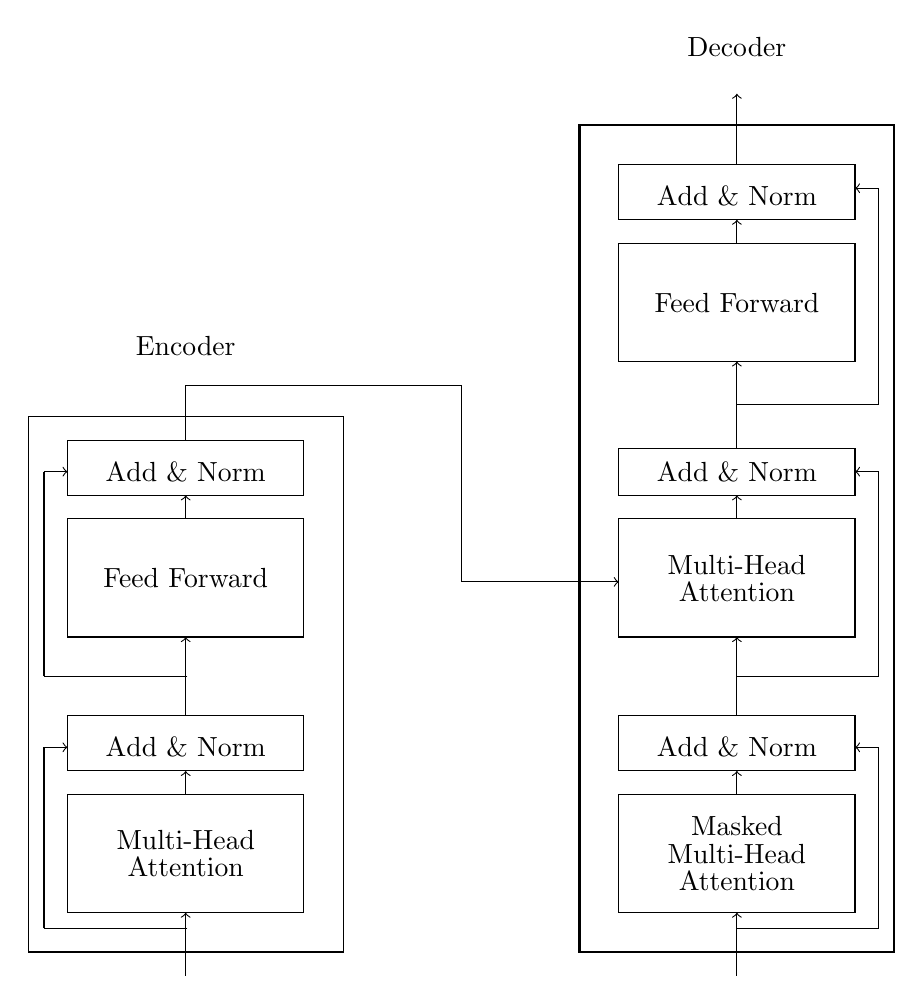
\begin{tikzpicture}[scale=1, transform shape]

        % Encoder
        \draw (0,0) rectangle (4,6.8);
        \node at (2,7.7) {Encoder};
        
        % Encoder components
        \draw (0.5,0.5) rectangle (3.5,2);
        \node at (2,1.25) {\shortstack{Multi-Head\\Attention}};
        
        \draw (0.5,2.3) rectangle (3.5,3);
        \node at (2,2.6) {Add \& Norm};
        
        \draw (0.5,4) rectangle (3.5,5.5);
        \node at (2,4.75) {Feed Forward};
        
        \draw (0.5,5.8) rectangle (3.5,6.5);
        \node at (2,6.1) {Add \& Norm};
        
        % Decoder
        \draw[thick] (7,0) rectangle (11,10.5);
        \node at (9,11.5) {Decoder};
        
        % Decoder components
        \draw (7.5,0.5) rectangle (10.5,2);
        \node at (9,1.25) {\shortstack{Masked\\Multi-Head\\Attention}};
        
        \draw (7.5,2.3) rectangle (10.5,3);
        \node at (9,2.6) {Add \& Norm};
        
        \draw (7.5,4) rectangle (10.5,5.5);
        \node at (9,4.75) {\shortstack{Multi-Head\\Attention}};
        
        \draw (7.5,5.8) rectangle (10.5,6.4);
        \node at (9,6.1) {Add \& Norm};
        
        \draw (7.5,7.5) rectangle (10.5,9);
        \node at (9,8.25) {Feed Forward};
        
        \draw (7.5,9.3) rectangle (10.5,10);
        \node at (9,9.6) {Add \& Norm};
        
        % Encoder lines
	\draw[->] (2, -0.3) -- (2, 0.5);
	\draw[->] (2, 2) -- (2, 2.3);
	\draw[->] (2, 3) -- (2, 4);
	\draw[->] (2, 5.5) -- (2, 5.8);
	\draw (2.02, 0.3) -- (0.2, 0.3);
	\draw (0.2, 0.3) -- (0.2, 2.6);
	\draw[->] (0.2, 2.6) -- (0.5, 2.6);

	\draw (2.02, 3.5) -- (0.2, 3.5);
	\draw (0.2, 3.5) -- (0.2, 6.1);
	\draw[->] (0.2, 6.1) -- (0.5, 6.1);

	% Decoder lines
	\draw[->] (9, -0.3) -- (9, 0.5);
	\draw[->] (9, 2) -- (9, 2.3);
	\draw[->] (9, 3) -- (9, 4);
	\draw[->] (9, 5.5) -- (9, 5.8);
	\draw[->] (9, 6.4) -- (9, 7.5);
	\draw[->] (9, 9) -- (9, 9.3);
	\draw[->] (9, 10) -- (9, 10.9);

	\draw (9, 0.3) -- (10.8, 0.3);
	\draw (10.8, 0.3) -- (10.8, 2.6);
	\draw[->] (10.8, 2.6) -- (10.5, 2.6);

	\draw (9, 3.5) -- (10.8, 3.5);
	\draw (10.8, 3.5) -- (10.8, 6.1);
	\draw[->] (10.8, 6.1) -- (10.5, 6.1); 

	\draw (9, 6.95) -- (10.8, 6.95);
	\draw (10.8, 6.95) -- (10.8, 9.7);
	\draw[->] (10.8, 9.7) -- (10.5, 9.7);


	\draw (2, 6.5) -- (2, 7.2);
	\draw (2, 7.2) -- (5.5, 7.2);
	\draw (5.5, 7.2) -- (5.5, 4.7);
	\draw[->] (5.5, 4.7) -- (7.5, 4.7);

        
    \end{tikzpicture}
    \caption{Esquema de la arquitectura de los transformers}
    \label{fig:transformers}
\end{figure}

La ide principal del transformer es, a lo largo de esta serie de capas, poder construir representaciones contextualizadas cada vez más acertadas de los significados de las palabras o \textit{tokens} de las secuencias de entrada. Así, en las distintas capas del transformer, para obtener la representación de una palabra, se combina la información de la representación obtenida en la capa anterior con la información de las representaciones de las palabras vecinas. El objetivo es producir la versión contextualizada de cada palabra, representando lo que significa esta en el contexto particular en que se encuentra. \cite{jurafsky2023speech}

A continuación se explica con más detalle los procesos que ocurren dentro de cada capa.

\subsection{Capas de \textit{multi-head attention}}
Las capas de \textit{multi-head attention} suponen la verdadera innovación de la arquitectura de transformers \cite{jurafsky2023speech}, pues es en estas donde el modelo aplica el mecansimo de atención.  En el caso de los transformers, se utiliza una variación del mecanismo de atención explicado en la sección \ref{atencion}. Esta variación se conoce como \textit{scaled dot-product attention}. Igual que en el mecanismo general de atención, se utilizan tres matrices: la matriz de \textit{queries} $Q$, la de claves $K$ (por su nombre en inglés, \textit{keys}) y la de valores $V$ (\textit{values}). En este caso, el valor de atención se calcula utilizando la siguiente fórmula:

\begin{equation}
A(Q, K, V) = softmax(\frac{QK^t}{\sqrt{d_k}})
\end{equation}

Donde $d_k$ es la dimensión del estado oculto de la fuente.

Como vemos, el cambio respecto al cálculo de atención descrito en la sección \ref{atencion} reside en que en este caso se añade el factor $\frac{1}{\sqrt{d_k}}$, que se utiliza para escalar el resultado obtenido, y conseguir así que las gradientes sean más estables, ya que si la secuencia de entrada fuera muy larga, la función \textit{softmax} puede devolver gradientes extremadamente pequeños, cosa que podria dificultar al modelo realizar un aprendizaje eficiente. \cite{multiheaddotproduct}

Aunque esta forma de cálculo de la atención es empleada por los transformers, estos no se quedan solamente en este concepto, sino que van un paso más allá y utilizan un tipo de atención algo más complejo conocido como \textit{multi-head attention}. Este proceso consiste en calcular distintas atenciones sobre las mismas \textit{queries} y pares clave-valor. Se utiliza este tipo de atención ya que las distintas palabras dentro de la secuencia de texto pueden estar relacionadas entre sí de muchas maneras distintas de manera simultánea. Capturar todas estas relaciones entre palabras es muy complicado si se utiliza un solo valor de atención.

Así, en las capas de \textit{multi-head attention} encontramos distintas capas de atención conocidas como \textit{heads} (cabezas), que calculan valores de atención de manera paralela. Cada una de estas tiene un conjunto distinto de parámetros que se aprende durante el entrenamiento, con los cuales hará el cálculo de atención entre las palabras de entrada. Utilizando parámetros distintos en cada cabeza se consigue que cada una se centre en aspectos distintos de las relaciones entre las palabras. El cálculo de atención para una cabeza $i$ se realiza mediante la siguiente fórmula:

\begin{equation}
H_i = A(QW_i^Q, KW_i^K, VW_i^V)
\end{equation}

Donde $W_i^Q$, $W_i^K$ y $W_i^V$ son las matrices de parámtetros asociadas a la \textit{query}, clave y valor respectivamente de la cabeza $i$. El valor de \textit{multi-head attention} se obtiene mediante la concatenación de los resultados de las cabezas. Para un total de $h$ cabezas de atención:

\begin{equation}
MultiHead(Q, K, V) = (H_1 \oplus H_2 \oplus ... \oplus H_h)W_O
\end{equation}

La matriz de parámetros $W_O$ proyecta la concatenación de los resultados de las $h$ cabezas de vuelta al subespacio original. \cite{cordonnier2021multiheadattentioncollaborateinstead, multiheaddotproduct, jurafsky2023speech}

\subsection{Caps de redes \textit{Feed Forward}}
Las capas de redes \textit{feed forward} en la arquitectura de transformers están compuestas por $N$ redes neuronales independientes de tipo \textit{feed forward} (en español, redes de propagación hacia adelante).

Una red neuronal de tipo \textit{feed forward} es una red multicapa en la que, a diferencia de las redes neuronales recurrentes (RNN) explicadas en la sección \ref{rnn}, las conexiones entre neuronas no pueden formar ciclos. Esto implica que las señales siempre se propagan en una única dirección: desde la capa de entrada hacia la capa de salida, pasando por las capas ocultas. En la arquitectura de transformers, estas redes están completamente conectadas, lo que significa que las neuronas de una capa reciben las salidas de todas las neuronas de la capa anterior y envían sus salidas a todas las neuronas de la capa siguiente. Además, típicamente contienen solamente una capa oculta.

Este tipo de red neuronal es similar al modelo de perceptró multicapa explicado en la sección \ref{perceptronmulticapa}, pero no deben confundirse, pues en el caso de las redes neuronales \textit{feed forward}, las unidades de cómputo no son perceptrones, sino unidades más complejas. \cite{jurafsky2023speech}

En los transformers, estas capas complementan las salidas de la capa de atención. Mientras que la capa de atención procesa cada palabra de la secuencia relacionandola con las demás palabras, las capas \textit{feef forward} procesan cada palabra de manera independiente. Este procesamiento es crucial para mejorar la representación de las características extraídas de la capa de atención.

\subsection{Capas de normalización}

Las capas de normalización se encuentran detrás de tanto las capas de atención como las de redes \textit{forward}. En ellas se aplica el proceso de normalización de capas (en inglés, \textit{layer normalization} o \textit{layer norm} \cite{ba2016layernormalization}). Este tipo de normalización se utiliza para mejorar el rendimiento del entrenamiento de redes neuronales profundas, manteniendo los valores de la capa oculta dentro de un rango que facilita el entrenamiento basado en gradientes.

El proceso de normalización de capas toma como entrada un vector para cada palabra de la secuencia, y devuelve este mismo vector normalizado. El primer paso en el proceso es calcular la media $\mu$ y la desviación típica $\sigma$ del vector, de la siguiente manera:

\begin{equation}
\mu^l = \frac{1}{H} \sum_{i = 1}^Hx_i^l
\end{equation}

\begin{equation}
\sigma^l = \sqrt{\frac{1}{H} \sum_{i = 1}^H (x_i^l - \mu^l)^2}
\end{equation}

Donde $H$ es el número de unidades ocultas en la capa. A continuación, los componentes del vector se normalizan restando la media y desviación típica calculadas \cite{jurafsky2023speech}:

\begin{equation}
\hat{x} = \frac{(x - \mu)}{\sigma}
\end{equation}

Finalmente, se introducen parámetros de \textit{bias} $b$ y \textit{gain} $g$:

\begin{equation}
LayerNorm = g\hat{x} + b
\end{equation}

%\section{Procesamiento del lenguaje natural} \label{nlp}

%El procesamiento de lenguaje natural (NLP, por su nombre en inglés \textit{Natural Language Processing}) es una rama de la inteligencia artificial que se ocupa del desarrollo de algoritmos y modelos para la realización de tareas relacionadas con el lenguaje humano. Más específicamente, involucra tareas como el modelado de lenguaje, clasificación de textos, recuperación y extracción de información, resumen de textos o traducción automática entre otras. \cite{alma997066713303706} 


\section{Modelos de lenguaje grandes}

%There are two existing strategies for applying pre-trained language representations to downstream tasks: feature-based and fine-tuning. The feature-based approach, such as ELMo (Peters et al., 2018a), uses task-specific architectures that include the pre-trained representations as additional features. The fine-tuning approach, such as the Generative Pre-trained Transformer (OpenAI GPT) (Radford et al., 2018), introduces minimal task-specific parameters, and is trained on the downstream tasks by simply fine-tuning all pretrained parameters. The two approaches share the same objective function during pre-training, where they use unidirectional language models to learn general language representations. \cite{devlin2019bertpretrainingdeepbidirectional}

%https://learning.oreilly.com/library/view/the-working-limitations/53863MIT65233/chapter001.xhtml#h1-1

Los modelos de lenguaje grandes (en inglés, \textit{Large Language Models} o LLM) son modelos de aprendizaje profundo basados en redes neuronales con miles de millones de parámetros, que utilizan la arquitectura de transformers. Estos modelos pueden ser entrenados con grandes cantidades de texto, perimitiéndoles realizar una gran cantidad de tareas en el ámbito del procesamiento de lenguaje natural.

Las tareas sobre las que se aplican son casos de generación condicional, es decir, generación de texto condicionado a un fragmento de entrada (\textit{prompt}), ya que los LLM son modelos que están diseñados fundamentalmente para predecir la siguiente palabra de una secuencia de palabras \cite{jurafsky2023speech}. Aunque el ámbito de tareas sobre el que se pueden aplicar los LLM pueda parecer reducido, la realidad es que la gran mayoría de tareas en el ámbito de NLP pueden ser enfocadas desde un punto de vista de generación condicional. Por ejemplo, para la tarea de responder preguntas, podriamos plantearlo de la siguiente manera:

En primer lugar, debemos proporcionar al modelo una \textit{prompt} con la pregunta a contestar, con un formato que sugiera que después de la pregunta se espera una respuesta, por ejemplo: 

\begin{displayquote}
\centerline{"Pregunta: ¿Cuál es la capital de Francia? Respuesta: "}
\end{displayquote}

A continuación, el modelo calcula la probabilidad para cada palabra $w$ dentro de su vocabulario de que esta sea la palabra que continua la \textit{prompt}:

\begin{displayquote}
\centerline{$P(w|\text{Pregunta: ¿Cuál es la capital de Francia? Respuesta: })$}
\end{displayquote}

Los vocabularios en los LLMs se refieren al conjunto de palabras sobre las que trabajan. Así, habiendo calculado las probabilidades para todas las posibles palabras, encontraremos algunas con probabilidades más altas, entre las cuales debería encontrarse la palabra \textit{París}, que es la respuesta a la pregunta. El modelo deberia seleccionar esta palabra y, si se quiere generar una respuesta más larga, se calcula la siguiente probabilidad:

\begin{displayquote}
\centerline{$P(w|\text{Pregunta: ¿Cuál es la capital de Francia? Respuesta: París})$}
\end{displayquote}

El proceso puede seguir hasta que llegemos al número de palabras deseadas.

Inicialmente, este cálculo de probabilidades se realizaba de manera secuencial, basando las predicciones en las distribuciones de probabilidad de las palabras dentro de un texto. Actualmente se utiliza la arquitectura de transformers, que permite procesar grandes cantidades de texto de manera eficiente y proporciona predicciones mucho más acertadas, pues tiene en cuenta el contexto en el que se encuentran las palabras y las relaciones entre estas \cite{burtsev2023working}.

Existen distintos enfoques para la selección de cuál es la palabra que sigue en la secuencia. Uno de los métodos más simples es utilizar el algoritmo de \textit{greedy decoding} \cite{gu2017trainablegreedydecodingneural}. El algoritmo \textit{greedy decoding} consiste en elegir la palabra con la probabilidad condicional más alta hasta el momento en cada instante.

\begin{equation}
\hat{w}_i = argmax_{w \in V} P(w | \{w_1, w_2, ..., w_{i-1}\})
\end{equation}

Con el tiempo se ha descubierto que este método llega a resultados subóptimos, pues al elegir siempre la palabra que es más probable que ocurra, tiende a generar textos excesivamente genéricos y repetitivos.

Existe una extension de este algoritmo conocida como \textit{beam search}, la cual ha demostrado ser más efectiva, sobretodo en tareas de traducción automática. La diferencia entre el algoritmo \textit{greedy decoding} y este, es que el \textit{beam search}, en lugar de quedarse solamente con la palabra con mayor probabilidad y crear una única respuesta, el algoritmo guarda $K > 1$ posibles respuestas (hipótesis) durante la decodificación. Así, en cada iteración, el algoritmo elige las K hipótesis con mayor \textit{score}:

\begin{equation}
\prod_{i = 1}^N = p(w_i | \{w_1, w_2, ..., w_{i-1}\})
\end{equation}

Cuando estas se terminan de generar, selecciona la hipótesis con mayor probabilidad logarítmica.

Aunque el rendimiento de \textit{beam search} es superior al \textit{greedy decoding}, en los LLM se suelen utilizar métodos más complejos, que proporcionan resultados más sofisticados. Estos métodos se conocen como métodos de generación por \textit{sampling}. Se explicarán con detalle en la siguiente sección.

\subsection{Métodos de generación por \textit{sampling}}

En términos generales, el proceso de \textit{sampling} consiste en seleccionar de manera aleatoria una serie de individuos de una muestra, teniendo (o no) en cuenta sus distribuciones de probabilidad. En el contexto de los LLM, esto se traduce en elegir las palabras que se generan en la secuencia de acuerdo con su probabilidad dentro del contexto definido por el modelo. De esta manera, es más probable seleccionar palabras con probabilidades altas y menos probable (aunque no imposible) elegir aquellas con probabilidades bajas.

 El algoritmo de generación por \textit{sampling} más sencillo se conoce como \textit{random sampling}, el cual consiste en seleccionar la siguiente palabra de la secuencia de de manera aleatoria según la distribución de probabilidades proporcionada por el transformer. Sin embargo, este enfoque es demasiado simplista para la generación de texto de calidad, ya que al seleccionar las palabras de manera aleatoria, incluso las palabras poco comunes, que tendrán probabilidades bajas, pueden ser elegidas, lo que podría resultar en la generación de frases incorrectas o extrañas \cite{jurafsky2023speech}.

Debido a estas limitaciones, en los LLM se suelen emplear algoritmos más sofisticados, los cuales analizaremos en las siguientes secciones.

\subsubsection{\textit{Top-k sampling}}

El algoritmo de \textit{top-k sampling} es una generalización del \textit{greedy decoding} que consiste en seleccionar las $K$ palabras con mayor probabilidad de la distribución y aplicar \textit{random sampling} únicamente sobre este conjunto. Una vez se seleccionan las $K$ palabras del conjunto, sus probabilidades deben ser normalizadas según el nuevo conjunto. Las probabilidades normalizadas se calculan de la siguiente manera:

\begin{equation}
\hat{p}_i = \frac{p_i * \mathbb{1}\{i \leq K\}}{\sum_{j = 1}^K p_j}
\end{equation}

Donde $\mathbb{1}$ es la función característica, que indica si una palabra está dentro o no del conjunto de las $K$ más probables \cite{nadeem2020systematiccharacterizationsamplingalgorithms}.

\subsubsection{\textit{Nucleus sampling}}

El algoritmo de \textit{nucleus sampling} \cite{holtzman2020curiouscaseneuraltext}, también conocido como \textit{top-p sampling} también sigue la idea de eliminar de la distribución las palabras menos probables. Sin embargo, en lugar de seleccionar un número fijo de palabras, lo que hace es mantener un el porcentaje $p$ más importante de la muestra. Así, dada una distribución $P(x |x_{1:i-1})$, las \textit{top-p} palabras del vocabulario $V^{(p)} \subset V$ se definen como el conjunto más pequeño que cumpla:

\begin{equation}
\sum_{x \in V^{(p)}} P(x | x_{1:i-1}) \ge p
\end{equation}

Al medir la probabilidad acumulada en lugar de un número fijo de palabras, se espera que esta medida sea más robusta incluso en contextos diversos, que podrian tener resultados muy distintos si se usara un número fijo de palabras. De nuevo, tras seleccionar el subconjunto de palabras del vocabulario se deben normalizar sus probabilidades.

Las probabilidades normalizadas de cada palabra en el vocabulario se pueden calcular como:

\begin{equation}
\hat{p}_i = \frac{p'_i}{\sum_{j = 1}^{|V|} p'_j}
\end{equation}

Donde $p'_i = p_i * \mathbb{1}\{\sum_{j = 1}^{i-1}p_j < P\}$ \cite{nadeem2020systematiccharacterizationsamplingalgorithms}.

\subsubsection{\textit{Tempered sampling}}

En el algoritmo de \textit{tempered sampling} \cite{nadeem2020systematiccharacterizationsamplingalgorithms} no crea un subconjunto de palabras del vocabulario, sino que ajusta la distribución de probabilidad de las palabras mediante una transformación. Para ello, se utiliza un parámetro $\tau$, que cumple $0 < \tau < 1$, según la siguiente fórmula:

\begin{equation}
\hat{p}_i = \frac{exp(log(p_i)/\tau)}{\sum_{j = 1}^{|V|}exp(log(p_j)/\tau)}
\end{equation}

Además, existe una variación de este algoritmo que se conoce como \textit{tempered top-k sampling}, el cual combina las transformaciones definidas por el algoritmo \textit{top-k} y el \textit{tempered sampling}. Así, la probabilidad normalizada se calcula:

\begin{equation}
\hat{p}_i = \frac{p'_i}{\sum_{j = 1}{|V|}p'_j}
\end{equation}

Donde $p'_i = exp(log(p_i)/\tau * \mathbb{1}\{i \leq K\}$ .

%En las siguientes secciones se presentan algunos de los modelos de lenguaje grandes más utilizados actualmente.

\subsection{Modelos de Lenguaje Grande Preentrenados (\textit{Pre-trained LLMs})} \label{pretrainedLLM}

Los modelos de lenguaje grandes preentrenados son modelos que han sido entrenados con grandes cantidades de datos generales, pero que aún no han sido ajustados para realizar tareas específicas. Este tipo de modelos han supuesto una revolución en el campo del procesamiento de lenguaje natural, ya que pueden ser adaptados para realizar una gran variedad de tareas específicas, incluso si estas difieren de los datos originales de entrenamiento. Utilizar LLMs preentrenados supone un ahorro de tiempo y recursos significativo, evitando la necesidad de entrenar un modelo desde cero con un gran conjunto de datos.

A continuación se presentan algunos de los modelos de lenguaje preentrenados más utilizados actualmente.

\subsubsection{GPT}

\subsubsection{Gemma}

\subsubsection{Llama-3}

\chapter{Adaptación de modelos de lenguaje grandes}

En este capítulo se aborda cómo podemos adaptar los modelos de lenguaje grandes (LLMs) preentrenados para realizar tareas específicas, explorando las diferentes estrategias y enfoques disponibles. Se hará especial incapié en el método PEFT (\textit{parameter-efficient fine-tuning}) y LoRA (\textit{Low-Rank Adaptation}).

\section{Ajuste de LLMs}

Tal y como se ha mencionado en la sección \ref{pretrainedLLM}, los LLMs preentrenados son modelos entrenados con grandes cantidades de datos genéricos que no han sido todavía ajustados para la realización de ninguna tarea específica. Por lo tanto, para aplicarlos a tareas concretas, es necesario ajustar estos modelos para adaptarlos a los requisitos específicos de cada tarea. Generalmente, para adaptar los modelos se utilizan técnicas de \textit{transfer learning}.

\subsection{Aprendizaje por transferencia}

El concepto de aprendizaje por transferencia (en inglés, \textit{transfer learning}) se refiere a la transferencia de conocimiento desde un dominio fuente, donde se dispone de una mayor cantidad de datos, hacia dominios más específicos, que cuentan con menos datos disponibles. Una definición formal dada en \cite{Weiss2016} es la siguiente:

\begin{displayquote}
\textit{"Dado un dominio fuente $D_s$ con una tarea fuente correspondiente $T_s$ y un dominio objetivo $D_t$ con una tarea correspondiente $T_t$, el aprendizaje por transferencia es el proceso de mejora de la función predictiva objetivo $f_t(\cdot)$ mediante el uso de la información relacionada del dominio $D_s$ y la tarea $T_s$, donde $D_s \neq D_t$ o $T_s \neq T_t$"}
\end{displayquote}

Existen cuatro enfoques principales dentro del aprendizaje por transferencia: aprendizaje basado en instancias (\textit{instance-based}), basado en características (\textit{feature-based}), basado en parámetros (\textit{parameter-based}) y basado en relaciones (\textit{relational-based}) \cite{Weiss2016}.

En cuanto al aprendizaje basado en instancias, la idea principal es utilizar una combinación de modelos preentrenados en el dominio fuente para etiquetar los datos no etiquetados del dominio objetivo. Para ello, se asignan pesos a los modelos del dominio fuente en función de su similitud con el dominio objetivo. Los resultados de los modelos se ponderan según estos pesos para estimar las etiquetas de los datos no etiquetados del dominio objetivo. Finalmente, se construye el modelo del dominio objetivo a partir de los datos etiquetados de este y las etiquetas estimadas.

En el enfoque basado en características, se crean nuevos modelos específicos para las tareas, y se incorpora en estos las representaciones obtenidas con el modelo preentrenado, añadiéndolas como características adicionales. De esta manera, el modelo preentrenado sirve como punto de partida para el modelo específico. Utilizando las características extraídas del modelo preentrenado, el modelo específico puede transferir el conocimiento general obtenido por este al contexto del dominio específico de la tarea. Dentro de este enfoque, existen dos variantes: asimétrico y simétrico  \cite{9134370}. En el enfoque asimétrico, se transforma las características extraídas por el modelo preentrenado para que se ajusten a las del dominio objetivo. Por el contrario, en el simétrico lo que se hace es buscar un espacio común de características latentes y transformar tanto las características del dominio fuente como del objetivo en una nueva representación de características.

En el enfoque basado en parámetros se modifica y reentrena el modelo preentrenado para la tarea en particular, ajustando directamente sus parámetros. De esta manera, el modelo conserva el conocimiento general obtenido en el preentrenamiento y, tras la modificación y reentrenamiento, aprende nuevo conocimiento específico de la tarea.

Por último, en el enfoque basado en relaciones se centra principalmente en los problemas de dominios relacionales, transfiriendo la lógica de relaciones o reglas aprendidas en el dominio fuente al dominio objetivo. Estos métodos buscan preservar y adaptar las relaciones entre entidades para resolver tareas en el nuevo dominio.

Para los experimentos de este trabajo, se realizará la adaptación de los modelos de lenguaje preentrenados mediante aprendizaje por tranferencia basado en parámetros. Específicamente, se utilizará la técnica de \textit{fine-tuning}.

El principal inconveniente del método de \textit{fine-tuning} es que puede ser un proceso muy lento, ya que es necesario ajustar todos los parámetros del modelo preentrenado, los cuales suelen ser numerosos. Existe un enfoque alternativo en el que se mantiene el modelo preentrenado intacto, y se añaden unos pocos parámetros adicionales que modifican su comportamiento interno para adaptarlo a la tarea específica. Durante el entrenamiento, solamente es necesario ajustar estos nuevos parámetros. Esta idea se conoce como adaptadores.

\section{Adaptadores}

El método de ajuste basado en adaptadores funciona añadiendo módulos específicos a un modelo preentrenado, de manera que durante el entrenamiento de este para alguna tarea específica se actualizan únicamente los parámetros de estos módulos, y no los del modelo completo. De esta manera, se incorporan solo unos pocos parámetros entrenables para cada nueva tarea, lo que permite un alto grado de compartición de parámetros \cite{he2021effectivenessadapterbasedtuningpretrained}. Este enfoque puede ser utilizado como alternativa al \textit{fine-tuning} completo del modelo, ya que, se ha demostrado que ambos métodos ofrecen un rendmiento comparable, siendo el ajuste con adaptadores mucho más eficientes en términos del número parámetros \cite{houlsby2019parameterefficienttransferlearningnlp, stickland2019bertpalsprojectedattention}.

Los módulos de los adaptadores deben cumplir con dos propiedades esenciales: contener un número reducido de parámetros y tener una incialización cercana a la identidad. los adaptadores deben ser pequeños en comparación con las capas del modelo original para asegurar que el modelo crezca de manera controlada al añadir nuevas tareas. La inicialización cercana a la unidad es necesaria para mantener la estabilidad del entrenamiento. De esta manera, el modelo original no se verá afectado al inicio del entrenamiento. Durante este, los adaptadores pueden activarse para cambiar la distribución de las activaciones en la red. Además, los módulos pueden ignorarse si no son necesarios. Si la incialización se desviara demasiado de la identidad, el modelo podria fallar durante el entrenamiento \cite{houlsby2019parameterefficienttransferlearningnlp}.

En el ámbito del procesamiento de lenguaje natural, los adaptadores generalmente se insertan como módulos entre las capas del modelo. En el caso de la arquitectura de transformers, la idea es insertar dos redes neuronales MLP poco profundas como cuello de botella dentro de cada uno de los bloques del transformer: una después de la capa de \textit{multi-head attention} y otra, después de la capa de red \textit{feed forward}. Estas redes MLP deben tener lo que se conoce como \textit{skip connections}, es decir, conexiones que permiten saltarse capas inermedias, para permitir la incialización de las redes como identidad \cite{murphy2022probabilistic}.

%Para la realización de este trabajo, se utilizará este método de ajuste basado en adaptadores, añadiendo específicamente módulos de PEFT (\textit{parameter-efficient fine-tuning}) y LoRA (\textit{Low-Rank Adaptation}).

\section{\textit{Parameter-efficient fine-tuning} (PEFT)}

Uno de los métodos de ajuste basado en adaptadores para los modelos de lenguaje grandes es el \textit{parameter-efficient fine-tuning} (PEFT).

Dentro de los métodos de \textit{fine-tuning} para LLM, PEFT (\textit{parameter-efficient fine-tuning}) es uno de los más eficientes, pues solamente requiere realizar el ajuste de unos pocos parámetros externos en lugar del LLM al completo, consiguiendo un rendimiento comparable o incluso mejor. \cite{hu2023llmadaptersadapterfamilyparameterefficient}

\section{\textit{Low-Rank Adaptation} (LoRA)}

%LoRA \cite{hu2021loralowrankadaptationlarge}

\chapter{Resultados experimentales}

\section{Conjunto de datos}

\section{Medidas de evaluación}

\section{Resultados experimentales}

????? ????????????? ????????????? ????????????? ????????????? ?????????????

%%%%%%%%%%%%%%%%%%%%%%%%%%%%%%%%%%%%%%%%%%%%%%%%%%%%%%%%%%%%%%%%%%%%%%%%%%%%%%%
%                                 CONCLUSIONS                                 %
%%%%%%%%%%%%%%%%%%%%%%%%%%%%%%%%%%%%%%%%%%%%%%%%%%%%%%%%%%%%%%%%%%%%%%%%%%%%%%%

\chapter{Conclusions}

????? ????????????? ????????????? ????????????? ????????????? ????????????? 

%%%%%%%%%%%%%%%%%%%%%%%%%%%%%%%%%%%%%%%%%%%%%%%%%%%%%%%%%%%%%%%%%%%%%%%%%%%%%%%
%                                BIBLIOGRAFIA                                 %
%%%%%%%%%%%%%%%%%%%%%%%%%%%%%%%%%%%%%%%%%%%%%%%%%%%%%%%%%%%%%%%%%%%%%%%%%%%%%%%

%%%%%%%%%%%%%%%%%%%%%%%%%%%%%%%%%%%%%%%%%%%%%%%%%%%%%%%%%%%%%%%%%%%%%%%%%%%%%%%
%                                BIBLIOGRAFIA                                 %
%%%%%%%%%%%%%%%%%%%%%%%%%%%%%%%%%%%%%%%%%%%%%%%%%%%%%%%%%%%%%%%%%%%%%%%%%%%%%%%

\bibliographystyle{plain}

\bibliography{plantillatfg}

\cleardoublepage

%%%%%%%%%%%%%%%%%%%%%%%%%%%%%%%%%%%%%%%%%%%%%%%%%%%%%%%%%%%%%%%%%%%%%%%%%%%%%%%
%                           APÈNDIXS  (Si n'hi ha!)                           %
%%%%%%%%%%%%%%%%%%%%%%%%%%%%%%%%%%%%%%%%%%%%%%%%%%%%%%%%%%%%%%%%%%%%%%%%%%%%%%%

\APPENDIX

%%%%%%%%%%%%%%%%%%%%%%%%%%%%%%%%%%%%%%%%%%%%%%%%%%%%%%%%%%%%%%%%%%%%%%%%%%%%%%%
%                         LA CONFIGURACIO DEL SISTEMA                         %
%%%%%%%%%%%%%%%%%%%%%%%%%%%%%%%%%%%%%%%%%%%%%%%%%%%%%%%%%%%%%%%%%%%%%%%%%%%%%%%

\chapter{Configuració del sistema}

????? ????????????? ????????????? ????????????? ????????????? ?????????????

\section{Fase d'inicialització}

????? ????????????? ????????????? ????????????? ????????????? ?????????????

\section{Identificació de dispositius}

????? ????????????? ????????????? ????????????? ????????????? ?????????????

%%%%%%%%%%%%%%%%%%%%%%%%%%%%%%%%%%%%%%%%%%%%%%%%%%%%%%%%%%%%%%%%%%%%%%%%%%%%%%%
%                               ALTRES  APÈNDIXS                              %
%%%%%%%%%%%%%%%%%%%%%%%%%%%%%%%%%%%%%%%%%%%%%%%%%%%%%%%%%%%%%%%%%%%%%%%%%%%%%%%


\chapter{??? ???????????? ????}

????? ????????????? ????????????? ????????????? ????????????? ????????????? 



%%%%%%%%%%%%%%%%%%%%%%%%%%%%%%%%%%%%%%%%%%%%%%%%%%%%%%%%%%%%%%%%%%%%%%%%%%%%%%%
%                              FI DEL DOCUMENT                                %
%%%%%%%%%%%%%%%%%%%%%%%%%%%%%%%%%%%%%%%%%%%%%%%%%%%%%%%%%%%%%%%%%%%%%%%%%%%%%%%

\end{document}
